% pdflatex  -synctex=1 -interaction=nonstopmode -file-line-error -recorder -output-directory="/mnt/c/Users/A613933/Documents/git/Master-Thesis/final-presentation"  "/mnt/c/Users/A613933/Documents/git/Master-Thesis/final-presentation/main.tex"'
\section{Kernel}

\begin{frame}[c]{}
    \begin{center}
        \textbf{A Linear Kernel for \psdom}

        \textit{Another Explicit kernel for a Dominating Problem}
    \end{center}
\end{frame}

\begin{frame}[c]{Kernelization}
\begin{itemize}
    \item \textbf{Idea: } Preprocess an instance using \textit{Reduction Rules} until hard \textit{kernel} is found.
\end{itemize}

\begin{figure}
\centering
\resizebox{0.35\textwidth}{!} {

\includegraphics{fig/pexels-yulia-ilina-10400351.jpg}
}
\end{figure}
\end{frame}


\begin{frame}[c]{Kernelization}
% Moreover, we require that $size_{\mathfrak{A}}(k) \leq g(k)$ for some computable function $g:\mathbb{N} \rightarrow \mathbb{N}$.


% \item A \textit{kernelization algorithm} or \textit{kernel} is an algorithm $\mathfrak{A}$ for a parameterized problem $Q$ that given an instance $(I,k)$ of $Q$ runs in polynomial time and returns an equivalent instance $(I', k')$ of $Q$. 
% A \underline{reduction rule} is a function $\phi:\Sigma^* \times \mathbb{N} \rightarrow \Sigma^* \times \mathbb{N}$ that maps an instance $(x,k)$ to an equivalent instance $(x',k')$ such that $\phi$ is computable in time polynomial in $\abs{x}$ and $k$.
%A reduction rule is \underline{sound} (or \underline{safe}) if $(I, k) \in Q \Leftrightarrow (I',k') \in Q$.

\begin{itemize}
    \item \textbf{Idea: } Preprocess an instance using \textit{Reduction Rules} until hard \textit{kernel} is found.
\end{itemize}

\pause \begin{figure}
\centering
\resizebox{0.5\textwidth}{!}{
    
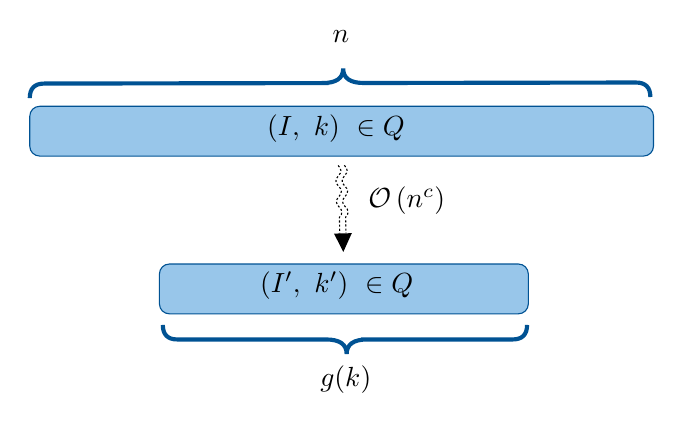
\begin{tikzpicture}[x=0.75pt,y=0.75pt,yscale=-1,xscale=1]
%uncomment if require: \path (0,290); %set diagram left start at 0, and has height of 290
\tikzset{every picture/.style={line width=0.75pt}} %set default line width to 0.75pt        

%Rounded Rect [id:dp2256907851376615] 
\draw  [color={rgb, 255:red, 0; green, 82; blue, 147 }  ,draw opacity=1 ][fill={rgb, 255:red, 152; green, 198; blue, 234 }  ,fill opacity=1 ] (129.8,74.8) .. controls (129.8,72.15) and (131.95,70) .. (134.6,70) -- (425.5,70) .. controls (428.15,70) and (430.3,72.15) .. (430.3,74.8) -- (430.3,89.2) .. controls (430.3,91.85) and (428.15,94) .. (425.5,94) -- (134.6,94) .. controls (131.95,94) and (129.8,91.85) .. (129.8,89.2) -- cycle ;
%Straight Lines [id:da34735862747158275] 
\draw  [dash pattern={on 0.75pt off 0.75pt}]  (281.37,98.46) .. controls (283.08,100.09) and (283.12,101.75) .. (281.49,103.46) .. controls (279.86,105.17) and (279.9,106.83) .. (281.61,108.46) .. controls (283.32,110.09) and (283.36,111.75) .. (281.73,113.46) .. controls (280.1,115.17) and (280.14,116.83) .. (281.85,118.46) .. controls (283.56,120.09) and (283.6,121.75) .. (281.97,123.46) -- (282.08,128.13) -- (282.15,131.13)(278.37,98.54) .. controls (280.08,100.16) and (280.12,101.82) .. (278.49,103.53) .. controls (276.86,105.24) and (276.9,106.9) .. (278.61,108.53) .. controls (280.32,110.16) and (280.36,111.82) .. (278.73,113.53) .. controls (277.1,115.24) and (277.14,116.9) .. (278.85,118.53) .. controls (280.56,120.16) and (280.6,121.82) .. (278.97,123.53) -- (279.08,128.21) -- (279.15,131.21) ;
\draw [shift={(280.87,140.17)}, rotate = 268.63] [fill={rgb, 255:red, 0; green, 0; blue, 0 }  ][line width=0.08]  [draw opacity=0] (8.93,-4.29) -- (0,0) -- (8.93,4.29) -- cycle    ;
%Rounded Rect [id:dp11606859634007116] 
\draw  [color={rgb, 255:red, 0; green, 82; blue, 147 }  ,draw opacity=1 ][fill={rgb, 255:red, 152; green, 198; blue, 234 }  ,fill opacity=1 ] (192.27,150.8) .. controls (192.27,148.15) and (194.42,146) .. (197.07,146) -- (365.2,146) .. controls (367.85,146) and (370,148.15) .. (370,150.8) -- (370,165.2) .. controls (370,167.85) and (367.85,170) .. (365.2,170) -- (197.07,170) .. controls (194.42,170) and (192.27,167.85) .. (192.27,165.2) -- cycle ;
%Shape: Brace [id:dp49500678764931805] 
\draw  [color={rgb, 255:red, 0; green, 82; blue, 147 }  ,draw opacity=1 ][line width=1.5]  (428.8,65.55) .. controls (428.79,60.88) and (426.46,58.55) .. (421.79,58.56) -- (290.81,58.79) .. controls (284.14,58.8) and (280.81,56.48) .. (280.8,51.81) .. controls (280.81,56.48) and (277.48,58.82) .. (270.81,58.83)(273.81,58.82) -- (136.79,59.06) .. controls (132.12,59.07) and (129.79,61.4) .. (129.8,66.07) ;
%Shape: Brace [id:dp39979872340961986] 
\draw  [color={rgb, 255:red, 0; green, 82; blue, 147 }  ,draw opacity=1 ][line width=1.5]  (193.9,175.35) .. controls (193.9,180.02) and (196.23,182.35) .. (200.9,182.35) -- (272.47,182.35) .. controls (279.14,182.35) and (282.47,184.68) .. (282.47,189.35) .. controls (282.47,184.68) and (285.8,182.35) .. (292.47,182.35)(289.47,182.35) -- (362.4,182.35) .. controls (367.07,182.35) and (369.4,180.02) .. (369.4,175.35) ;

% Text Node
\draw (242.9,72.9) node [anchor=north west][inner sep=0.75pt]    {$( I,\ k) \ \in Q$};
% Text Node
\draw (291.67,107.4) node [anchor=north west][inner sep=0.75pt]    {$\mathcal{O}\left( n^{c}\right)$};
% Text Node
\draw (239.5,148.4) node [anchor=north west][inner sep=0.75pt]    {$( I',\ k') \ \in Q$};
% Text Node
\draw (268.5,193.9) node [anchor=north west][inner sep=0.75pt]    {$g( k)$};
% Text Node
\draw (274.5,32.4) node [anchor=north west][inner sep=0.75pt]    {$n$};


\end{tikzpicture}

}
\end{figure}
\end{frame}

\begin{frame}[c]{Related Works}
    \centering
    \resizebox{0.8\textwidth}{!}{
        \begin{tabularx}{\textwidth}{lcX}
            \textbf{Problem} & \textbf{Size}   & \textbf{Source}       \\
            \pdom            & $67k$           &~\cite{Diekert2005}    \\
            \ptdom           & $410k$          &~\cite{Garnero2018}    \\
            \psdom           & $359 k$ & \textbf{This work}    \\
                             &                 &                       \\
            \peddom          & $14k$           &~\cite{Guo2007} \\
            \pefdom          & $84k$           &~\cite{Guo2007} \\
            \prbdom          & $43k$           &~\cite{Garnero2017}    \\
            \pcdom           & $130k$          &~\cite{Luo2013}        \\
            \pdirdom         & Linear          &~\cite{Alber2006}      \\
        \end{tabularx}
    }
\end{frame}


%\subsection{Definitions}
\begin{frame}[c]{Main Theorem}
\begin{tcolorbox}[colback=TUMBlueLighter,title=The Main Theorem]
    \psdom parameterized by solution size admits a linear kernel.
    There exists a polynomial-time algorithm that, given a planar graph $(G, k)$, either correctly reports that $(G, k)$ is a NO-instance or returns an equivalent instance $(G', k)$ such that $|V(G')| \leq 359 \cdot k$.
\end{tcolorbox}
\end{frame}

\begin{frame}[c]{The Big Picture}
    Given a planar graph $G = (V ,E)$, we will:

    \begin{enumerate}
     \pause   \item Split the neighborhoods of the graph;
     \pause   \item Define reduction Rules
     \pause   \item Use the region decomposition to analyze the size of each region
    \end{enumerate}
\end{frame}
%%%% REGIONS DEFINITION

\subsection{Definitions}
\begin{frame}[c]{The Basic Principle: Regions}
    % Introduced by Alber et al.~\cite{Alber2004}, decomposition technique for planar graph.

    \begin{tcolorbox}[colback=TUMBlueLighter,title=Region (Simplified)]
        Given plane $G$ and $v,w \in V$, a region is a closed subset, such that
        \begin{itemize}
            \item there are two non-crossing (but possibly overlapping) boundary paths
            \item Every vertex in R belongs to $N(v,w)$
        \end{itemize}
    \end{tcolorbox}
    \pause \begin{figure}[!ht]
            \resizebox{0.35\textwidth}{!}{
                \tikzfig{./img/region-base}
            }
        \end{figure}
\end{frame}

\begin{frame}[c]{The Basic Principle: Regions}

    \begin{tcolorbox}[colback=TUMBlueLighter,title=Region (Simplified)]
        Given plane $G$ and $v,w \in V$, a region is a closed subset, such that
    \begin{itemize}
        \item there are two non-crossing (but possibly overlapping) boundary paths
        \item Every vertex in R belongs to $N(v,w)$
    \end{itemize}
    \end{tcolorbox}

    \begin{figure}[!ht]
    \resizebox{0.35\textwidth}{!}{
         \tikzfig{./img/region-single}
    }
    \end{figure}
\end{frame}

\begin{frame}[c]{\dreg}
    \begin{tcolorbox}[colback=TUMBlueLighter,title={\dreg\cite{Alber2004}}]
        Given $G = (V, W)$ and $D \subseteq V$, a \dreg is a set $\mathfrak{R}$ with poles in $D$ such that:
        \begin{itemize}
            \item for any $vw$-region $R \in \mathfrak{R}$: $D \cap V(R) = \{v, w\}$
            \item Regions are disjunct, but can share border vertices
        \end{itemize}
    \end{tcolorbox}
   \pause A region is \textbf{maximal}, if no $R \in \mathfrak{R}$ such that $\mathfrak{R}' = \mathfrak{R} \cup \{R\}$ is a \dreg with $V(\mathfrak{R})\subsetneq V(\mathfrak{R}')$.
\end{frame}

\begin{frame}[c]{Maximal \dreg}
    \begin{figure}[!ht]
        \resizebox{0.55\textwidth}{!}{
            \tikzfig{./img/region}
        }
    \end{figure}
\end{frame}

\begin{frame}[c]{Splitting Up $N(v)$}
    \begin{figure}[!ht]
        \resizebox{0.5\textwidth}{!}{
            \tikzfig{../thesis/fig/tikz/neighborhoods-single-vertex}
        }
    \end{figure}
\end{frame}
\begin{frame}[c]{Splitting Up $N(v)$}
 %Let \G be a graph and let $v \in V$. 
 We split $N(v)$ into three subsets:
    \begin{align}
       \pause N_1(v) & = \{u \in N(v) : N(u) \setminus N[v] \neq \emptyset \}              \\
        \pause N_2(v) & = \{u \in N(v)\setminus N_1(v) : N(u) \cap N_1(v) \neq \emptyset \} \\
        \pause N_3(v) & = N(v) \setminus (N_1(v) \cup N_2(v))
    \end{align}
    For $i,j \in [1,3]$, we denote $N_{i,j} (v) := N_i(v) \cup N_j(v)$. 
    %Furthermore, we call a vertex $v'$ \textit{confined} by a vertex $v$, if $N(v') \subseteq N[v]$.
\end{frame}


\subsection{Rule 1}
\begin{frame}[c]{Rule 1: Shrinking $N_3(v)$}

    \begin{tcolorbox}[colback=TUMBlueLighter,title=]
        Let \G be a graph and let $v \in V$. If $|N_3(v)| \geq 1$:
        \begin{itemize}
            \item remove $N_{2,3}(v)$ from G,
            \item add a vertex $v'$ and an edge $\{v, v'\}$.
        \end{itemize}
    \end{tcolorbox}

    \begin{figure}[!ht]
    \resizebox{0.4\textwidth}{!}{
         \tikzfig{../thesis/fig/tikz/ruleone}
    }
    \end{figure}
    \begin{itemize}
        \item \textbf{Idea: } $v$ better choice than $N_{2,3}$
    \end{itemize}
\end{frame}

\begin{frame}[c]{Splitting up $N(v,w)$}

    \begin{figure}[!ht]
        \resizebox{0.7\textwidth}{!}{
            \tikzfig{../thesis/fig/tikz/neighborhoods-two-vertices}
        }
    \end{figure}
\end{frame}

\begin{frame}[c]{Splitting up $N(v,w)$}
    \begin{align}
      \pause  N_1(v,w) & = \{u \in N(v,w) \mid N(u) \setminus (N(v,w)\cup \{v,w\}) \neq \emptyset \}  \\
      \pause  N_2(v,w) & = \{u \in N(v,w)\setminus N_1(v,w) \mid N(u) \cap N_1(v,w) \neq \emptyset \} \\
      \pause  N_3(v,w) & =  N(v,w) \setminus (N_1(v,w) \cup N_2(v,w))
    \end{align}
    For $i,j \in [1,3]$, we denote $N_{i,j}(v,w) = N_i(v,w) \cup N_j(v,w)$.
\end{frame}


\begin{frame}[c]{Rule 2: Setting Up Our Weapons}
    \textbf{Key Idea: } $N_{2,3}(v, w)$ can \textbf{always} be semitotally dominated with 4 vertices.
    \pause\begin{align}
        \Dvw & = \{ \tilde D \subseteq N_{2,3}(v,w)            \mid N_3(v,w) \subseteq \bigcup_{v \in \tilde D} N(v),\ |\tilde D| \leq 3                  \} \\
        \Dv  & = \{ \tilde D \subseteq N_{2,3}(v,w) \cup \{v\} \mid N_3(v,w) \subseteq \bigcup_{v \in \tilde D} N(v),\ |\tilde D| \leq 3,\ v \in \tilde D \} \\
        \Dw  & = \{ \tilde D \subseteq N_{2,3}(v,w) \cup \{w\} \mid N_3(v,w) \subseteq \bigcup_{v \in \tilde D} N(v),\ |\tilde D| \leq 3,\ w \in \tilde D \}
    \end{align}

\end{frame}

\begin{frame}[c]{Rule 2}
    If $\mathbf{\Dvw = \emptyset}$ we apply the following:

    \begin{caseof}
       \case{if $\Dv =  \emptyset$ and $D_w = \emptyset$}

        \begin{itemize}
            \item Remove $N_{2,3}(v,w)$
            \item Add vertices $v'$ and $w'$ and two edges $\{v, v'\}$ and $\{w, w'\}$
            \item Preserve $d(v,w)$
        \end{itemize}
        \pause \case{if $\Dv \neq  \emptyset$ and $D_w = \emptyset$}

        \begin{itemize}
            \item Remove $N_{2,3}(v)$
            \item Add $\{v, v'\}$
        \end{itemize}
        
        \pause \case{if $\Dv =  \emptyset$ and $D_w \neq \emptyset$} Symmetric
    \end{caseof}
\end{frame}

\subsection{Rule 2}
\begin{frame}[2]{Rule 2: Case 1}
    \begin{figure}[!ht]
    \resizebox{0.9\textwidth}{!}{
         \tikzfig{./img/rule2-case1}
    }
\end{figure}
\end{frame}

\begin{frame}[2]{Rule 2: Case 2}
    \begin{figure}[!ht]
    \resizebox{0.9\textwidth}{!}{
         \tikzfig{./img/rule2-case2}
    }
\end{figure}
\end{frame}

\begin{frame}[c]{Simple Regions}

    \begin{tcolorbox}[colback=TUMBlueLighter,title=The Main Theorem]
        A simple $vw$-region is a $vw$-region such that:
        \begin{enumerate}
            \item its boundary paths have length at most 2, and
            \item $V(R) \setminus \{v,w\} \subseteq N(v) \cap N(w)$.
        \end{enumerate}
    \end{tcolorbox}

    \pause\begin{figure}[!ht]
        \resizebox{0.35\textwidth}{!}{
            \tikzfig{../thesis/fig/tikz/simple-region-example}
        }
    \end{figure}

\end{frame}

\subsection{Rule 3}
\begin{frame}[c]{Rule 3: Shrinking the Size of Simple Regions}

Let \G be a plane graph, $v, w \in V$ and $R$ be a simple region between $v$ and $w$. If $|V(R) \setminus \{v, w\}| \geq 5$ apply the following:

\begin{caseof}
        \case{If $G[R\setminus\partial R] \cong P_3$, then:}

            \begin{itemize}
                    \item remove $V(R\setminus\partial R)$
                    \item add vertex $y$ with edges $\{v, y\}$ and $\{y, w\}$
            \end{itemize}

        \case{If $G[R\setminus\partial R] \ncong P_3$, then}

            \begin{itemize}
                    \item remove $V(R\setminus\partial R)$
                    \item add vertices $y$, $y'$ and four edges $\{v,y\}$, $\{v, y'\}$, $\{y, w\}$ and $\{y', w\}$
            \end{itemize}
        \end{caseof}
\end{frame}

\begin{frame}[c]{Rule 3: Shrinking the Size of Simple Regions}

    \begin{caseof}
        {\bfseries
        \case{If $G[R\setminus\partial R] \cong P_3$, then:}

            \begin{itemize}
                    \item remove $V(R\setminus\partial R)$
                    \item add vertex $y$ with edges $\{v, y\}$ and $\{y, w\}$
            \end{itemize}
        }

        \case{If $G[R\setminus\partial R] \ncong P_3$, then}

            \begin{itemize}
                    \item remove $V(R\setminus\partial R)$
                    \item add vertices $y$, $y'$ and four edges $\{v,y\}$, $\{v, y'\}$, $\{y, w\}$ and $\{y', w\}$
            \end{itemize}
        \end{caseof}

    \begin{figure}[!ht]
    \resizebox{0.35\textwidth}{!}{
         \tikzfig{./img/rulethree-1}
    }
    \end{figure}
\end{frame}

\begin{frame}[c]{Rule 3: Shrinking the Size of Simple Regions}

    \begin{caseof}
        \case{If $G[R\setminus\partial R] \cong P_3$, then:}

            \begin{itemize}
                    \item remove $V(R\setminus\partial R)$
                    \item add vertex $y$ with edges $\{v, y\}$ and $\{y, w\}$
            \end{itemize}
        {\bfseries
        \case{If $G[R\setminus\partial R] \ncong P_3$, then}

            \begin{itemize}
                    \item remove $V(R\setminus\partial R)$
                    \item add vertices $y$, $y'$ and four edges $\{v,y\}$, $\{v, y'\}$, $\{y, w\}$ and $\{y', w\}$
            \end{itemize}
        }
        \end{caseof}

    \begin{figure}[!ht]
    \resizebox{0.35\textwidth}{!}{
         \tikzfig{./img/rulethree-2}
    }
    \end{figure}
\end{frame}


\begin{frame}[c]{Notes}
    \begin{itemize}
        \pause \item We proved that all these rules are sound,
        \pause \item change the solution size by only a constant factor
        \pause \item and can be applied in poly-time.
    \end{itemize}
\end{frame}

\subsection{Kernel Size}
% ANIMATING BOUND
\begin{frame}[c]{Bounding the Kernel: Vertices Outside any Region}   
    \begin{figure}[!ht]
    \resizebox{0.35\textwidth}{!}{
         \tikzfig{./img/bounding-1}
    }
    \end{figure}

    \pause For each $d$ in sds $D$:
    \begin{enumerate}
           \pause \item $|N_1(v) \setminus V(\mathfrak{R})| = 0$~\cite{Alber2004}, On Border
           \pause \item $|N_2(v) \setminus V(\mathfrak{R})| = 96$~\cite{Alber2004}: TODO Reasoning  
           \pause \item $|N_3(v) \setminus V(\mathfrak{R})| = 1$, by Rule 1
        \end{enumerate}
\end{frame}
\begin{frame}[c]{Bounding the Kernel: Inside a region}

    \begin{figure}[!ht]
    \resizebox{0.35\textwidth}{!}{
         \tikzfig{./img/bounding-2}
    }
    \end{figure}
    For each $vw$-region, we have
    \begin{enumerate}
\pause        \item $|N_1(v,w)| \leq 4$~\cite{Alber2004} (vertices on border)
\pause        \item $|N_2(v,w)| \leq 6 \cdot 4$ (simple regions to $N_1(v,w)$, Rule 3)
\pause        \item $|N_3(v,w)| \leq \max(27,44,4,57) \cdot 4$ (proof omitted depending on Rule 2)
    \end{enumerate}

    \textbf{Total: } $|V(R)| = |\{v, w\} \cup (N_1(v,w) \cup N_2(v, w) \cup N_3(v, w))| \leq 87$
\end{frame}
\begin{frame}[c]{Bounding the Kernel: Number of Regions}

    \begin{figure}[!ht]
    \resizebox{0.35\textwidth}{!}{
         \tikzfig{./img/bounding-3}
    }

    \end{figure}
    \pause\begin{tcolorbox}[colback=TUMBlueLighter,title=Number of Regions~\cite{Alber2004}]
        Let G be a plane graph and let $D$ be a \sdom with $|D| \geq 3$. There is a maximal \dreg of $G$ sucht that $|\mathfrak{R}| \leq 3 \cdot |D|- 6$.
    \end{tcolorbox}

\end{frame}

\begin{frame}[c]{Summary: Bounding Kernel Size}

    Let D be sds of size $k$. There exists a maximal \dreg $\mathfrak{R}$ such that:

    \begin{enumerate}
        \item $\mathfrak{R}$ has only at most $3 k - 6$ regions (\cite{Alber2004});
        \item There are at most $97 \cdot k$ vertices outside of any region;
        \item Each region  $R \in \mathfrak{R}$ contains at most $87$ vertices.
    \end{enumerate}

    \textbf{Hence: } $|V| = \bigcup_{v \in D} N(v) = 87 \cdot (3k - 6) + 97 \cdot k + k < 359 \cdot k$

\end{frame}

\begin{frame}[c]{Main Theorem}
    All reduction rules can be applied in poly/time, hence:

\begin{tcolorbox}[colback=TUMBlueLighter,title=The Main Theorem]
    The \sdom problem parameterized by solution size admits a linear kernel on planar graphs.
    There exists a polynomial-time algorithm that, given a planar graph $(G, k)$, either correctly reports that $(G, k)$ is a NO-instance or returns an equivalent instance $(G', k)$ such that $|V(G')| \leq 359 \cdot k$.
\end{tcolorbox}
\textbf{Proof: } Add Proof here.
\end{frame}

